% Chapter 2
\chapter{Mathematical Background } % Main chapter title

\label{Chapter2} % For referencing the chapter elsewhere, use \ref{Chapter2} 

\lhead{Chapter 2. \emph{Mathematical Background}} % This is for the header on each page - perhaps a shortened title

%----------------------------------------------------------------------------
\section*{Overview}

This chapter is dedicated to provide mathematical notions necessary for under
standing the intuition behind manifold learning. Further, we present the
most representative manifold learning algorithms which are used in this thesis to solve specific problems in image processing and anomaly detection. We follow the structure from  Nicolas Thorstensen \citep{Thor2009} and Boothby \citep{Boot2003}. 
 
%----------------------------------------------------------------------------------------
\section{Metric Space}
Use of near and far is intuitive yet rigorous at the same time, which is rare in mathematics. Classifying the relationship between two 'primitives', whether they are close or far apart is some time not useful for the computation. A metric space is the mathematical construct of redefining the near and far primitive idea, which is useful in computation.


\begin{definition}

A metric on an arbitrary abstract set $\mathbb{X}$ is a function $d:\mathbb{X}\times \mathbb{X}\to [0,\infty)$ such that for all $a,b,c\in \mathbb{X}$, the following conditions are satisfied:

\begin{enumerate}
\item Non-negativity:	$d(a,b)\geq 0 and d(a,b)=0\Leftrightarrow a=b$
\item Symmetry:	$d(a,b)=d(b,a)$
\item Triangle inequality:  $d(a,c)\leq d(a,b)+d(b,c)$
	
\end{enumerate}

Then we say that $d$ is a \emph{metric} on $\mathbb{X}$ and that $(\mathbb{X},d)$ is a \emph{metric space}.

\end{definition}

A quite known instance of a metric space is the three dimensional
Euclidean space $\mathbb{R}^3$ with the Euclidean metric.


\begin{definition}\label{D;norm}
Let $V$ be a vector space over ${\mathbb R}$ and $N:V\rightarrow{\mathbb R}$ a map such that, $N({\mathbf v})=\|{\mathbf v}\|$, the following condition holds:
 
(i) Non-negativity: $\|{\mathbf v}\|\geq 0$ for all ${\mathbf v}\in V$. If $\|{\mathbf v}\|=0$, then ${\mathbf v}={\boldsymbol 0}$.

(ii) Linearity: If $\lambda\in{\mathbb R}$ and ${\mathbf v}\in V$,
then $\|\lambda{\mathbf v}\|=|\lambda| \|{\mathbf v}\|$.

(iii)Triangle inequality: If ${\mathbf v_1},\,{\mathbf v_2}\in V$, then 
$\|{\mathbf v_1}\|+\|{\mathbf v_2}\|\geq \|{\mathbf v_1}+{\mathbf v_2}\|$.

\noindent Then we call $\|\ \|$ a \emph{norm} and say that
$(V,\|\ \|)$ is a \emph{normed vector space}.
\end{definition}

Any normed vector space can be made into a metric space by the condition $d({\mathbf v_1},{\mathbf v_2})= \|{\mathbf v_1}-{\mathbf v_2}\|$.

\begin{definition}\label{D;inner product}
Let $V$ be a vector space over ${\mathbb R}$
and $M:V\times V\rightarrow{\mathbb R}$ a map such that,
writing $M({\mathbf v_1},{\mathbf v_2})
=\langle{\mathbf v_1},{\mathbf v_2}\rangle$, 
the following results
hold for ${\mathbf v_1},\,{\mathbf v_2},\,{\mathbf v_3}\in V$,
$\lambda\in{\mathbb R}$.

(i) $\langle{\mathbf v_1},{\mathbf v_2}\rangle\geq 0$.

(ii) If  $\langle{\mathbf v_1},{\mathbf v_2}\rangle=0$, then 
${\mathbf v_1}={\boldsymbol 0}$.

(iii)  $\langle{\mathbf v_1},{\mathbf v_2}\rangle
=\langle{\mathbf v_1},{\mathbf v_2}\rangle$.

(iv) $\langle{\mathbf v_1}+{\mathbf v_3},{\mathbf v_2}\rangle
=\langle{\mathbf v_1},{\mathbf v_2}\rangle
+\langle{\mathbf v_3},{\mathbf v_2}\rangle$.

(v) $\langle\lambda {\mathbf v_1},{\mathbf v_2}\rangle
=\lambda\langle{\mathbf v_1},{\mathbf v_2}\rangle$.

\noindent Then we call $\langle\ ,\  \rangle$ an 
\emph{inner product} and say that
$(V,\langle\ ,\  \rangle)$ is an \emph{inner product space}.
\end{definition}

Working on ${\mathbb R}^{n}$ to make it vector space, then 
$\langle{\mathbf x},{\mathbf y}\rangle=\sum_{j=1}^{n}x_{j}y_{j}$
is an inner product. We notice that the norm derived from inner product is called Euclidean norm.

\section{Topology}

With the metric structure in hand, the idea of 'near' and 'far' between elements of metric space can be quantified by characterizing the connectivity
of sets through small neighborhoods of elements which gives rise to a topology of the sets.

\begin{definition}
Let $(\mathbb{X},d)$ be a metric space and element $x \in \mathbb{X}$. If $r>0$, then $B_{open}(x,r)=\{y\,:\,d(x,y)<r\}$ is called as \emph{open ball} 
with centre ${\mathbf x}$ and radius $r$. Similarly, $B_{closed}(x,r)=\{y\,:\,d(x,y)\leq r\}$ is called closed ball.
\end{definition}

The topology of $\mathbb{X}$ induce by the
metric is easy to study. 

\begin{definition}\label{topology}
Let $\mathbb{X}$ be a set and $\tau$ a collection of subsets of $\mathbb{X}$ 
with the following properties.

(i) The empty set $\emptyset\in \tau$ and the space $\mathbb{X}\in\tau$.

(ii) If $U_{\alpha}\in\tau$ for all $\alpha\in A$, then
$\bigcup_{\alpha\in A} U_{\alpha}\in\tau$.

(iii) If $U_{j}\in\tau$ for all $1\leq j\leq n$, then
$\bigcap_{j=1}^{n} U_{j}\in\tau$.

Then we say that $\tau$ is a \emph{topology} on $\mathbb{X}$ and
that $(\mathbb{X},\tau)$ is a \emph{topological space}. 
\end{definition}

If $(\mathbb{X},d)$ is a metric space, then the collection of open sets forms a topology. The topology of a set allows one to study properties such as connectivity.

\subsection{Connectedness}

The metric space $(\mathbb{X}, d)$ is not connected if it is the union of two disjoint open nonempty sets. Similarly, the converse of earlier implies that $(\mathbb{X}, d)$ is connected. Mathematically, It can be defined as:

\begin{definition}\label{disconnected} 
A topological space $(\mathbb{X},\tau)$ is said to be \emph{disconnected} if we can find non-empty
open sets $V_1$ and $V_2$ such that $V_1\cup V_2=\mathbb{X}$
and $V_1\cap V_2=\emptyset$. A space which is not disconnected is called \emph{connected}.
\end{definition}

\subsection{Neighborhoods}

Hausdorff was the first one to define topologies in terms of neighborhoods. It always appears to be technically easier to define topologies in terms of open sets as we have been doing it so far. Generally, It can be defined as:
\begin{definition}\label{neighbourhood} 
Let $(\mathbb{X},\tau)$ be a topological space. If $x\in \mathbb{X}$, we say that $N$ is a \emph{neighbourhood} of $x$ if we can find $U\in\tau$ with $x\in U\subseteq N$.
\end{definition}

\section{Manifolds}
A manifold is a topological space that locally resembles Euclidean space near each point. More precisely, they are spaces that locally look like the much more familiar Euclidean spaces. This allows the well-understood notions on Euclidean spaces to be generalised to manifolds rather directly. Using all the above definition, we now define manifold.

\begin{definition}
A $d$-dimensional manifold is a topological space \ref{topology} in which 
points can be separated by neighborhoods \ref{neighbourhood} and where every point has a neighborhood that is homeomorphically mapped onto an open Euclidean ddimensional ball \citep{Thor2009}.
\end{definition}

As the general definition is not apt to perform vector calculus on a manifold, The the notion of a differentiable manifold comes hand in hand with the concept of coordinate chart \ref{chart}. It can be thought of as assigning a set of coordinates to the points in the neighborhood $U$.

\begin{figure}[ht]
\begin{center}
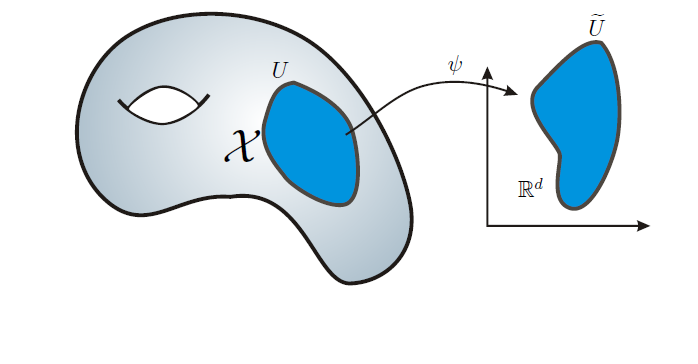
\includegraphics[width=\textwidth]{./Figures/chart.png}
\caption{Coordinate Chart\citep{Ety2008}}
\label{chart}
\end{center}
\end{figure}

To provide an entire description  of the manifold, several chart over manifold is used rather single. Transition map with two chart, corresponds to a change of coordinates is depicted in the figure \ref{TM}. 

\begin{figure}[ht]
\begin{center}
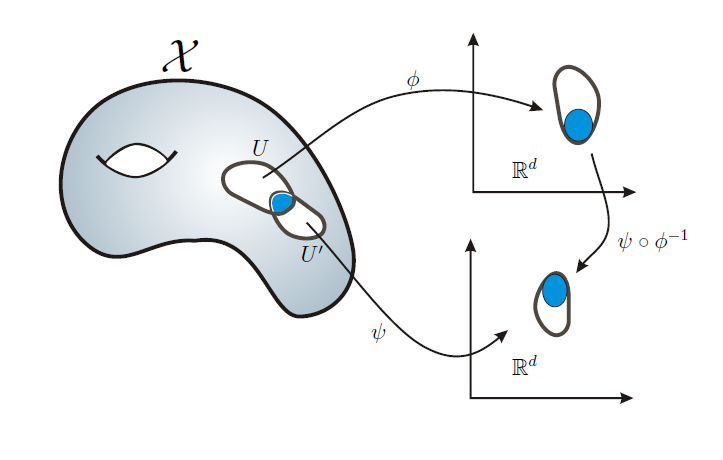
\includegraphics[width=\textwidth]{./Figures/TM.png}
\caption{Transition map.\citep{Ety2008}}
\label{TM}
\end{center}
\end{figure}

\section{Tangent Spaces}
The notion of linear approximation of a surface in vector calculus translates
to tangent space in differential geometry. The tangent space to a manifold $\mathcal{X}$ at a point $x$ is the closest flat approximation to $\mathcal{X}$ at that point.  If the dimension of $\mathcal{X}$ is $n$, then the tangent space is an $\mathbb{R}^n$ grazing $\mathcal{X}$ at $x$, as shown in figure \ref{tangent}. For detail discussion please refer work by Nicolas Thorstensen \citep{Thor2009} and Boothby \citep{Boot2003}.

\begin{figure}[ht]
\begin{center}
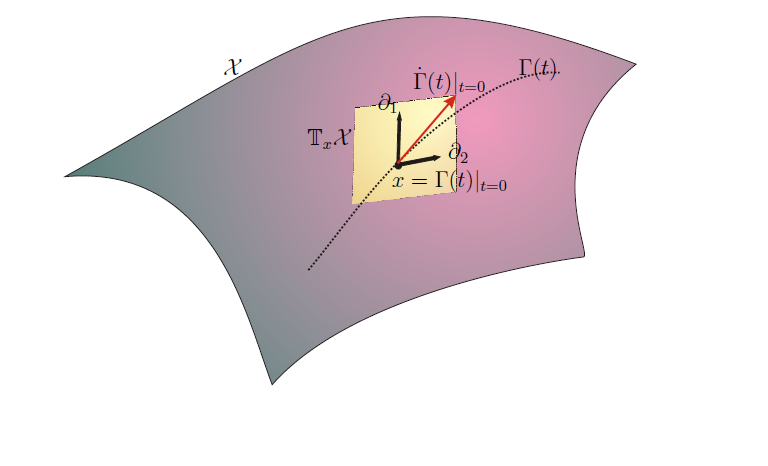
\includegraphics[width=\textwidth]{./Figures/tangent.png}
\caption{Tangent Space.\citep{Ety2008}}
\label{tangent}
\end{center}
\end{figure}

\subsection{Embedding}

When talking about the relationship between two topological objects, it is interesting to imagine a mapping from one object to the other that somehow preserves its original properties.

Let $\mathbb{X}$ and $\mathbb{Y}$ be two topological objects of the same type, a function $\phi \colon \mathbb{X} \to \mathbb{Y}$ is an embedding of $\mathbb{X}$ into $\mathbb{Y}$ if $\phi$ is an isomorphism which preserves the original properties of $\mathbb{X}$, where such properties are relative to the type of the objects at hand. Shortly, $\mathbb{X}$ is said to be \textit{embedded} in $\mathbb{Y}$.

\begin{example}[Embedding of Spaces]
	Consider the vector spaces $\mathbb{R}^p$ and $\mathbb{R}^q, p \leq q, p > 0$ and the isomorphism $t \colon \mathbb{R}^q \to \mathbb{R}^t \mid t(x) = [x | \bar{0}] = y$, where $y$ is the vector $x$ concatenated with $p-q$ zeros. $\mathbb{R}^p$ is embedded on $\mathbb{R}^q$, as the operations sum and scalar multiplication are preserved.
\end{example}

The same definition applies to manifolds too.